\documentclass[12pt]{article}
\usepackage{amsmath}
\usepackage{amssymb}
\usepackage{graphicx}
\usepackage{physics}
\usepackage{siunitx}
\usepackage{wrapfig}

\AtBeginDocument{\RenewCommandCopy\qty\SI}
\newcommand{\E}[1]{\times 10^{#1}}

\begin{document}
    \DeclareSIUnit{\atm}{atm}
    \DeclareSIUnit{\cal}{\ cal}
    \DeclareSIUnit{\Cal}{\ Cal}
    \DeclareSIUnit{\calorie}{\ cal}
    \DeclareSIUnit{\Calorie}{\ Cal}
    \DeclareSIUnit{\celsiusdegree}{C^\circ}
    \DeclareSIUnit{\fahrenheit}{^\circ F}
    \DeclareSIUnit{\torr}{\ torr}

    \section{Problem 1}
        Find the mass in kilograms of $7.50 \times 10^{24}$ atoms of arsenic, which has a molar mass of $74.9 \unit{\gram/\mole}$.

        \subsection{Solution}
            Convert atoms to moles.
            \begin{equation}
                \frac{7.50 \times 10^{24} \text{ atoms}}{6.02 \times 10^{23} \text{ atoms/mol}} = 12.458 \unit{\mole}
            \end{equation}

            Using the molar mass, convert moles to grams.
            \begin{equation}
                12.458 \unit{\mole} * 74.9 \unit{\gram/\mole} = 933.140 \unit{\gram} = \boxed{0.933 \unit{\kilo\gram}}
            \end{equation}

    \pagebreak
    \section{Problem 3}
        Oxygen gas having a volume of $1000 \unit{\centi\meter^3}$ at $40.0\unit{\celsius}$ and $1.01 \times 10^5 \unit{\pascal}$ expands until its volume is $1500 \unit{\centi\meter^3}$ and its pressure is $1.06 \times 10^5 \unit{\pascal}$. 
        Find (a) the number of moles of oxygen present and (b) the final temperature of the sample.

        \subsection{Solution (a)}
            We can use the ideal gas law for this.
            We apply it to the first case, converting the 40.0\unit{\celsius} to Kelvin.
            \begin{align}
                40\unit{\celsius}   &=  313.15 \unit{\kelvin}\\
                1000 \unit{\centi\meter^3}  &=  1000 \times 10^{-6} \unit{\meter^3} = 1 \times 10^{-3} \unit{\meter^3}\\
                pV  &=  nRT\\
                n   &=  \frac{pV}{RT}
                    =   \frac{1.01 \times 10^5 \unit{\pascal} * 10^{-3} \unit{\centi\meter^3}}{8.31 \unit{\joule/\mole\cdot\kelvin} * 313.15 \unit{\kelvin}}\\
                    &=  \frac{1.01 \times 10^2 \unit{\newton \cdot \meter}}{2602.2765 \unit{\joule/\mole}}
                    =   \boxed{0.038812 \unit{\mole}}
            \end{align}

        \subsection{Solution (b)}
            The ideal gas law (or an equivalent) will be used here.
            The number of moles does not change here, neither does the gas constant $R$. 
            We can use ths to solve for the final value of the temperature.
            \begin{gather}
                \frac{p_1 V_1}{n_1 T_1} =   \frac{p_2 V_2}{n_2 T_2}\\
                \frac{p_1 V_1}{T_1} =   \frac{p_2 V_2}{T_2}\\
                T_2 =   T_1 * \frac{p_2 V_2}{p_1 V_1}
            \end{gather}

            We can substitute in values now.
            \begin{align}
                T_2 &=  T_1 * \frac{p_2 V_2}{p_1 V_1}
                    =   313.15 * \frac{1.06 \times 10^5 * 1500}{1.01 \times 10^5 * 1000}\\
                    &=  313.15 * \frac{1.06 * 1.5}{1.01}
                    =   \boxed{492.97 \unit{\kelvin} \approx 220 \unit{\celsius}}
            \end{align}

    \pagebreak
    \section{Problem 5}
        The best laboratory vacuum has a pressure of about $1.00 \times 10^{-18} \unit{\atm}$, or $1.01 \times 10^{-13} \unit{\pascal}$. 
        How many gas molecules are there per cubic centimeter in such a vacuum at 293 K?

        \subsection{Solution}
            Use the ideal gas law, the version with Boltzmann's constant.
            We can solve for $\frac{N}{V}$.
            \begin{gather}
                pV  =   NkT\\
                \frac{N}{V} =   \frac{p}{kT}
            \end{gather}

            From here, we can just plug and chug, so to speak.
            \begin{align}
                \frac{N}{V} &=  \frac{1.01 \times 10^{-13} \unit{\newton/\meter^2}}{1.38 \times 10^{-23} \unit{\newton\cdot\meter/\kelvin} * 293 \unit{\kelvin}}
                    =   \frac{1.01 \times 10^{10}}{404.34} \unit{\meter^{-3}}\\
                    &=  24978978.09 \times \unit{\meter^{-3}}
                    =   \boxed{24.979 \unit{\centi\meter^{-3}}}
            \end{align}

    \pagebreak
    \section{Problem 7}
        Suppose 1.80 mol of an ideal gas is taken from a volume of 3.00 \unit{\meter^3} to a volume of 1.50 \unit{\meter^3} via an isothermal compression at 30\unit{\celsius}. 
        (a) How much energy is transferred as heat during the compression, and (b) is the transfer to or from the gas?

        \subsection{Solution (a)}
            Energy transfered can be thought of as work. 
            We have a formula for work done by an ideal gas.
            \begin{equation}
                W   =   nRT \ln\left( \frac{V_f}{V_i} \right)
            \end{equation}

            We can plug and chug into this.
            \begin{align}
                T_K &=  T_C + 273.15 \unit{\kelvin}
                    =   30 \unit{\celsius} + 273.15 \unit{\kelvin}
                    =   303.15 \unit{\kelvin}\\
                W   &=  (1.80 \unit{\mole}) (8.31 \unit{\joule/\mole}) (303.15 \unit{\kelvin}) \ln\left( \frac{1.5 \unit{\meter^3}}{3.0 \unit{\meter^3}} \right)\\
                    &=  4534.5177 \unit{\joule} * (-0.693147)
                    =   -3143.088 \unit{\joule}
            \end{align}

            The energy transfered is the absolute value of this, which would be \boxed{3143.088 \unit{\joule}}. 

        \subsection{Solution (b)}
            This is a volume compression process.
            The total energy in the system would remain constant, so $Q = W$ by the first law of thermodynamics.
            This means $Q < 0$, so the energy is transfered \boxed{from} the gas as heat.

    \pagebreak
    \section{Problem 9}
        An automobile tire has a volume of $1.64 \times 10^{-2} \unit{\meter^3}$ and contains air at a gauge pressure (pressure above atmospheric pressure) of 165 kPa when the temperature is 0.00\unit{\celsius}. 
        What is the gauge pressure of the air in the tires when its temperature rises to 27.0\unit{\celsius} and its volume increases to $1.67 \times 10^{-2} \unit{\meter^3}$? 
        Assume atmospheric pressure is $1.01 \times 10^5 \unit{\pascal}$.

        \subsection{Solution}
            We can here use the ideal gas law.
            \begin{gather}
                pV = nRT\\
                \frac{p_1 V_1}{T_1} =   \frac{p_2 V_2}{T_2}
            \end{gather}

            With our equation, we solve for $p_f$. 
            \begin{gather}
                p_f =   p_i \frac{V_i T_f}{V_f T_i}
            \end{gather}

            This can be ``plugged-and-chugged'' to find our final answer.
            We should also bear in mind that the gauge pressure should be added to the atmospheric pressure to find the overall pressure.
            Do not forget to convert to Kelvin.
            \begin{align}
                T_{iK}  &=  0 \unit{\celsius} + 273 \unit{\kelvin}
                    =   273 \unit{\kelvin}\\
                T_{fK}  &=  27 \unit{\celsius} + 273 \unit{\kelvin}
                    =   300 \unit{\kelvin}\\
                p_i &=  p_{gauge} + p_{atm}
                    =   165 \times 10^3 \unit{\pascal} + 1.01 \times 10^5 \unit{\pascal}
                    =   266 \times 10^3 \unit{\pascal}\\
                p_f &=  p_i \frac{V_i T_f}{V_f T_i}
                    =   266 \times 10^3 \unit{\pascal} * \frac{(1.64 \times 10^{-2} \unit{\meter^3}) (300 \unit{\kelvin})}{(1.67 \times 10^{-2} \unit{\meter^3}) (273 \unit{\kelvin})}\\
                    &=  266 \times 10^3 \unit{\pascal} * \frac{492}{455.91}
                    =   287 \times 10^3 \unit{\pascal}
            \end{align}

            This can in turn be turned into the gauge pressure (our final answer) by subtracting the atmospheric pressure.
            \begin{equation}
                p_{gauge;f} =   287 \times 10^{3} \unit{\pascal} - 1.01 \times 10^5 \unit{\pascal}
                    =   \boxed{1.86 \times 10^5 \unit{\pascal}}
            \end{equation}

    \pagebreak
    \section{Problem 11}
        Air that initially occupies $0.140 \unit{\meter^3}$ at a gauge pressure of $103.0 \unit{\kilo\pascal}$ is expanded isothermally to a pressure of $101.3 \unit{\kilo\pascal}$ and then cooled at constant pressure until it reaches its initial volume. 
        Compute the work done by the air. 
        Gauge pressure is the difference between the actual pressure and atmospheric pressure.

        \subsection{Solution}
            Isothermal expansion means that there is no net change in energy, so $Q_{in} = W_{out}$ (a.k.a. $Q_{in} = -W_{in}$) as volume increases. 
            There is a formula for work we can use.
            \begin{equation}
                W = \int_{V_i}^{V_f} p(V)\,dV
            \end{equation}

            The problem outright states that it is separated into two parts: the isothermal expansion at changing pressure and the cooling at constant pressure.
            We can separate our equation into these two parts and find useful equations for each.
            The integrals will be separated at a point of $V = V_{max}$ since that is the point where the volume reachest its highest.
            We can call the final pressure value of $101.3 \unit{\kilo\pascal}$ the value $p_r$, with no meaning to its name.
            \begin{align}
                W   &=  \int_{V_i}^{V_f} p(V)\,dV
                    =   \int_{V_i}^{V_{max}} p_1(V)\,dV + \int_{V_{max}}^{V_f} p_2(V)\,dV\\
                    &=  \int_{V_i}^{V_{max}} \frac{nRT_i}{V} \,dV + \int_{V_{max}}^{V_f} p_r\,dV\\
                    &=  nRT_i \ln\left( \frac{V_{max}}{V_i} \right) + \int_{V_{max}}^{V_f} p_r\,dV\\
                    &=  p_i V_i \ln\left( \frac{V_{max}}{V_i} \right) + p_r (V_f - V_{max})
            \end{align}
            
            This requires the initial and maximum magnitudes of the volume, of which we only have one. 
            We can use the ideal gas law to find that which we need.
            First solve for the final volume, given $n$, $R$, and $T$ are constant.
            Do not forget to convert gauge pressure to overall pressure by adding the atmospheric pressure ($1.01 \times 10^5 \unit{\pascal}$).
            We can assume that the final pressure is not gauge pressure.
            \begin{gather}
                \begin{align}
                    p_i &=  p_1 + p_{atm}
                        =   103.0 \times 10^3 + 1.01 \times 10^5 \unit{\pascal}
                        =   2.04 \times 10^5 \unit{\pascal}\\
                    p_f &=  p_2 % + p_{atm}
                        =   101.3 \times 10^3 \unit{\pascal} % + 1.01 \times 10^5 \unit{\pascal}
                        % =   2.023 \times 10^5 \unit{\pascal}
                \end{align}\\
                pV  =   nRT\\
                p_i V_i =   p_f V_f =   p_f V_{max}\\
                \begin{align}
                    V_{max} &=  V_i * \frac{p_i}{p_f}
                        =   0.140 \unit{\meter^3} * \frac{2.04 \times 10^5 \unit{\pascal}}{1.013 \times 10^5 \unit{\pascal}}
                        =   0.281935 \unit{\meter^3}
                \end{align}
            \end{gather}

            This can in turn be applied to our above equation for the work done by the gas.
            {\footnotesize
            \begin{align}
                W   &=  p_i V_i \ln\left( \frac{V_{max}}{V_i} \right) + \int_{V_{max}}^{V_f} p_r\,dV\\
                    &=  0.140 \unit{\meter^3} * 2.04 \times 10^5 \unit{\pascal} * \ln\left( \frac{0.281935 \unit{\meter^3}}{0.140 \unit{\meter^3}} \right)
                            + \int_{0.281935 \unit{\meter^3}}^{0.140 \unit{\meter^3}} 1.013 \times 10^5 \unit{\pascal} \,dV\\
                    &=  28560 * 0.7000 + 101300 * (-0.1419)
                    =   19992.96 \unit{\joule} - 14378 \unit{\joule}\\
                    &=  \boxed{5614.95 \unit{\joule}}
            \end{align}}


    \pagebreak
    \section{Problem 13}
        \begin{wrapfigure}{r}{0.25\textwidth}
            \vspace{-30pt}
            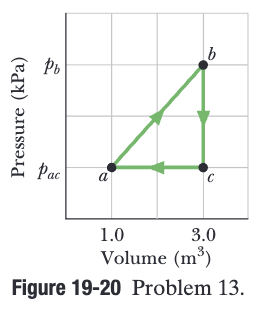
\includegraphics[width=0.25\textwidth]{picture_19-20.png} 
            % \label{fig:wrapfig}
        \end{wrapfigure}
        A sample of an ideal gas is taken through the cyclic process $abca$ shown in Fig. 19-20. 
        The scale of the vertical axis is set by $p_b = 7.5\,\unit{\kilo\pascal}$ and $p_{\rm ac} = 2.5\,\unit{\kilo\pascal}$. 
        At point $a$, $T = 200\,\unit{\kelvin}$.
        (a) How many moles of gas are in the sample? 
        What are (b) the temperature of the gas at point $b$, (c) the temperature of the gas at point $c$, and (d) the net energy added to the gas as heat during the cycle?

        \subsection{Solution (a)}
            We can use the ideal gas law.
            We need to solve for $n$ at point $a$. 
            \begin{gather}
                pV  =   nRT \to n   =   \frac{pV}{RT}
            \end{gather}

            From here, we plug in values to find $n$.
            \begin{align}
                n   &=  \frac{(2.5\,\unit{\kilo\pascal}) * (1.0\,\unit{\meter^3})}{R (200\,\unit{\kelvin})}
                    =   \frac{2.5 \times 10^3\,\unit{\joule}}{1662\,\unit{\joule/\mole}}
                    =   \boxed{1.504\,\unit{\mole}}
            \end{align}

        \subsection{Solution (b)}
            We can use the ideal gas law again, this time comparing two situations and finding the final temperature.
            \begin{gather}
                \frac{p_i V_i}{T_i} =   \frac{p_f V_f}{T_f} \to
                    T_f =   T_i * \frac{p_f V_f}{p_i V_i}
            \end{gather}

            From here, we plug in values to find the final temperature.
            \begin{align}
                T_f &=  T_i * \frac{p_f V_f}{p_i V_i}
                    =   200\,\unit{\kelvin} * \frac{7.5\,\unit{\kilo\pascal} * 3.0\,\unit{\meter^3}}{2.5\,\unit{\kilo\pascal} * 1.0\,\unit{\meter^3}}\\
                    &=  200\,\unit{\kelvin} * 9
                    =   \boxed{1800\,\unit{\kelvin}}
            \end{align}

        \subsection{Solution (c)}
            Use the ideal gas law again.
            This time, the pressure does not change.
            \begin{gather}
                \frac{V_i}{T_i} =   \frac{V_f}{T_f} \to
                    T_f =   T_i * \frac{V_f}{V_i}
            \end{gather}

            Now, we plug in to find $T_f$.
            \begin{align}
                T_f &=  T_i * \frac{V_f}{V_i}
                    =   1800\,\unit{\kelvin} * \frac{1.0\,\unit{\meter^3}}{3.0\,\unit{\meter^3}}
                    =   \boxed{600\,\unit{\kelvin}}
            \end{align}

        \subsection{Solution (d)}
            Let's start by calculating the total work done by the gas.
            We can separate it based on the phases.
            The phase between points b and c has no change in volume, so no work is done.
            \begin{align}
                W   &=  \int p(V)\,dV\\
                    &=  \int_{1.0 \unit{\meter^3}}^{3.0 \unit{\meter^3}} V * 2500\,\unit{\pascal/\meter^3}\,dV
                        +   \int_{3.0 \unit{\meter^3}}^{3.0 \unit{\meter^3}} p_{\rm bc}\,dV
                        +   \int_{3.0 \unit{\meter^3}}^{1.0 \unit{\meter^3}} 2500 \unit{\pascal}\,dV\\
                    &=  (1250\,\unit{\pascal/\meter^3}) \left( \frac{(3.0 \unit{\meter^3})^2 - (1.0 \unit{\meter^3})^2}{2} \right)
                        +   2500 \unit{\pascal} * (-2.0 \unit{\meter^3})\\
                    &=  4 * 2500\,\unit{\joule} - 2 * 2500 \unit{\joule}
                    =   10000 - 5000\,\unit{\joule}
                    =   5000\,\unit{\joule}
            \end{align}

            Since the this is a cyclical process, we can apply the firat law of thermodynamics.
            \begin{gather}
                \Delta E_{\rm int}  =   0   =   Q_{\rm in} - W_{\rm out}\\
                Q_{\rm in}  =   W_{\rm out} =   \boxed{5000\,\unit{\joule}}
            \end{gather}

    \pagebreak
    \section{Problem 17}
        \begin{wrapfigure}{r}{0.25\textwidth}
            \vspace{-30pt}
            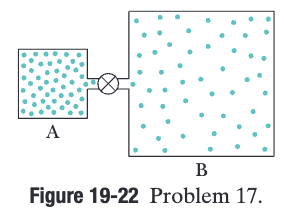
\includegraphics[width=0.25\textwidth]{picture_19-22.png} 
            % \label{fig:wrapfig}
        \end{wrapfigure}
        Container A in Fig. 19-22 holds an ideal gas at a pressure of $5.0 \times 10^5\,\unit{\pascal}$ and a temperature of 300 K. 
        It is connected by a thin tube (and a closed valve) to container B, with four times the volume of A. 
        Container B holds the same ideal gas at a pressure of $1.0 \times 10^5\,\unit{\pascal}$ and a temperature of 400 K. 
        The valve is opened to allow the pressures to equalize, but the temperature of each container is maintained. 
        What then is the pressure?

        \subsection{Solution}
            Let's put together a formulas for the number of moles of the ideal gas in each container (A and B). 
            We can use the Ideal Gas Law for this.
            \begin{align}
                n_A &=  \frac{p_A V_A}{R T_A}
                    =   \frac{5.0 \times 10^5\,\unit{\pascal} * V_A}{R * 300\,\unit{\kelvin}}
                    =   \frac{5 \times 10^3}{3} * \frac{V_A}{R}\\
                n_B &=  \frac{p_B V_B}{R T_B}
                    =   \frac{1.0 \times 10^5\,\unit{\pascal} * 4 V_A}{R * 400\,\unit{\kelvin}}
                    =   1 \times 10^3 * \frac{V_A}{R}
            \end{align}

            We can combine these to find the total number of moles.
            \begin{align}
                n_{\Sigma}  &=  n_A + n_B
                    =   \left( \frac{5}{3} + 1 \right) \times 10^3 * \frac{V_A}{R}
                    =   \frac{8}{3} \times 10^3 * \frac{V_A}{R}
            \end{align}

            We also know the total volume that there is.
            \begin{gather}
                V_{\Sigma}  =   \sum V_i
                    =   V_A + V_B
                    =   V_A + 4V_A
                    =   5V_A
            \end{gather}

            We can also calculate the average temperature of the cobined system, weighted by the volumes.
            \begin{align}
                T_{\rm avg} &=  \frac{\sum V_i * T_i}{\sum V_i}
                    =   \frac{V_A * T_A + V_B * T_B}{5V_A}\\
                    &=  \frac{V_A * 300\,\unit{\kelvin} + 4 V_A * 400\,\unit{\kelvin}}{5V_A}\\
                    &=  \frac{300\,\unit{\kelvin} + 1600\,\unit{\kelvin}}{5}
                    =   \frac{1900\,\unit{\kelvin}}{5}
                    =   380\,\unit{\kelvin}
            \end{align}

            We have our final values for the number of moles, volume, and temperature, not to mention that $R$ is a constant.
            We can put these into the ideal gas law to find the pressure at this point, assuming the pressure to be even.
            \begin{align}
                pV  &=  nRT\\
                p   &=  \frac{nRT}{V}
                    =   \frac{\frac{8}{3} \times 10^3 * \frac{V_A}{R} * R * 380\,\unit{\kelvin}}{5V_A}\\
                    &=  \left( \frac{8}{15} \times 10^3 * 380 \right)\,\unit{\pascal}
                    =   \boxed{2.03 \times 10^5 \unit{\pascal}}
            \end{align}

    \pagebreak
    \section{Problem 19}
        (a) Compute the rms speed of a nitrogen molecule at 20.0\unit{\celsius}. 
        The molar mass of nitrogen molecules ($N_2$) is given in Table 19-1.
        At what temperatures will the rms speed be (b) half that value and (c) twice that value?

        \subsection{Solution (a)}
            As stated in table 19-1, the molar mass of Nitrogen gas ($N_2$) molecules is $28.0 \times 10^{-3}\,\unit{\kilo\gram/\mole}$. 
            We can use that to find the molecule's rms (root-mean-square) speed.
            \begin{align}
                T_{K}   &=  T_{\unit{\celsius}} + 273 \unit{\kelvin}
                    =   293\,\unit{\kelvin}\\
                v_{\rm rms} &=  \sqrt{\frac{3RT}{M}}
                    =   \sqrt{\frac{3 * 8.31\,\unit{\joule/\mole\cdot\kelvin} * 293\,\unit{\kelvin}}{28.0 \times 10^{-3}\,\unit{\kilo\gram/\mole}}}\\
                    &=  \sqrt{\frac{7304.49}{28.0} \times 10^{3}\,\unit{\meter^2/\second^2}}
                    =   \boxed{510.8\,\unit{\meter/\second}}
            \end{align}
        
        \subsection{Solution (b)}
            We can use the same equation, this time solving for the temperature.
            \begin{gather}
                \frac{v_{\rm rms}}{2}   =   \sqrt{\frac{3 * 8.31\,\unit{\joule/\mole\cdot\kelvin} * T}{28.0 \times 10^{-3}\,\unit{\kilo\gram/\mole}}}\\
                \frac{3 * 8.31\,\unit{\joule/\mole\cdot\kelvin} * 293\,\unit{\kelvin}}{28.0 \times 10^{-3}\,\unit{\kilo\gram/\mole}} * \frac{1}{4} =   \frac{3 * 8.31\,\unit{\joule/\mole\cdot\kelvin} * T}{28.0 \times 10^{-3}\,\unit{\kilo\gram/\mole}}\\
                T   =   \frac{293\,\unit{\kelvin}}{4}
                    =   73.25\,\unit{\kelvin}
                    =   \boxed{-199.75\,\unit{\celsius}}
            \end{gather}
        
        \subsection{Solution (c)}
            The same equation can be used.
            \begin{gather}
                2 v_{\rm rms}   =   \sqrt{\frac{3 * 8.31\,\unit{\joule/\mole\cdot\kelvin} * T}{28.0 \times 10^{-3}\,\unit{\kilo\gram/\mole}}}\\
                \frac{3 * 8.31\,\unit{\joule/\mole\cdot\kelvin} * 293\,\unit{\kelvin}}{28.0 \times 10^{-3}\,\unit{\kilo\gram/\mole}} * 4 =   \frac{3 * 8.31\,\unit{\joule/\mole\cdot\kelvin} * T}{28.0 \times 10^{-3}\,\unit{\kilo\gram/\mole}}\\
                T   =   4 * 293\,\unit{\kelvin} 
                    =   1172\,\unit{\kelvin}
                    =   \boxed{899\,\unit{\celsius}}
            \end{gather}

    \pagebreak
    \section{Problem 23}
        A beam of hydrogen molecules ($H_2$) is directed toward a wall, at an angle of $55\unit{\degree}$ with the normal to the wall. 
        Each molecule in the beam has a speed of $1.0\,\unit{\kilo\meter/\second}$ and a mass of $3.3 \times 10^{-24} \unit{\gram}$. 
        The beam strikes the wall over an area of $2.0 \unit{\centi\meter^2}$, at the rate of $10^{23}$ molecules per second. 
        What is the beam's pressure on the wall?

        \subsection{Solution}
            This solution may be difficult to understand because $p$ represents both pressure and momentum.
            We need more letters.
            Maybe we could look at some language with a lot of different letters/characters.
            My Chinese teacher says their language has about 1500.
            We have a formula for pressure exerted by an ideal gas.
            \begin{equation}
                p   =   \frac{nMv_{\rm rms}^2}{3V}  =   \frac{F}{A}
            \end{equation}

            We assume that any collision of a molecule with a wall is fully elastic, so we can find a formula for the change in the vertical momentum.
            This would only be for a single particle and we will only be considering the horizontal velocity.
            \begin{align}
                v_i &=  v_{\rm rms} * \sin(55\unit{\degree})\\
                v_f &=  -v_i\\
                \Delta p    &=  p_f - p_i
                    =   mv_f - mv_i\\
                    &=  2mv_f
                    =   -2m * v_{\rm rms} * \cos(55\unit{\degree})
            \end{align}

            This can be multiplied by the rate at which the molecules hit the wall to find the total force, which is itself constant.
            \begin{align}
                F   &=  p * \dv{N}{t}
                    =   -2m * v_{\rm rms} * \cos(55\unit{\degree}) * 10^{23}\,\unit{\second^{-1}}
            \end{align}

            We can apply this to our equation for the pressure.
            That would be the final equation that we can plug values into.
            \begin{align}
                p   &=  \frac{F}{A}
                    =   -\frac{2m * v_{\rm rms} * \cos(55\unit{\degree}) * 10^{23} \unit{\second^{-1}}}{A}\\
                    &=  -\frac{2 * 3.3 \times 10^{-27}\,\unit{\kilo\gram} * 1000\,\unit{\meter/\second} * \cos(55\unit{\degree}) * 10^{23}\,\unit{\second^{-1}}}{2.0 \times 10^{-4}\,\unit{\meter^2}}\\
                    &=  -1893 \unit{\pascal}
            \end{align}

            Since pressure is always positive, we can finalize this by taking the absolute value to get our final answer.
            Said answer would be \boxed{1893\,\unit{\pascal}}. 

    \pagebreak
    \section{Problem 25}
        Determine the average value of the translational kinetic energy of the gas's molecules of an ideal gas at temperatures (a) 0.00\unit{\celsius} and (b) 100\unit{\celsius}.
        What is the translational kinetic energy per mole of an ideal gas at (c) 0.00\unit{\celsius} and (d) 100\unit{\celsius}?

        \subsection{Solution (a)}
            The average translational kinetic energy is determined by a simple formula, which we can use here.
            \begin{equation}
                K   =   \frac{3}{2} kT
                    =   \frac{3}{2} * 1.38\E{-23}\,\unit{\joule/\kelvin} * 273\,\unit{\kelvin}
                    =   \boxed{565.11\E{-23}\,\unit{\joule}}
            \end{equation}

        \subsection{Solution (b)}
            Same strategy.
            \begin{equation}
                K   =   \frac{3}{2} kT
                    =   \frac{3}{2} * 1.38\E{-23}\,\unit{\joule/\kelvin} * 373\,\unit{\kelvin}
                    =   \boxed{772.11\E{-23}\,\unit{\joule}}
            \end{equation}

        \subsection{Solution (c)}
            The kinetic energy of a system (in this case a mole of atoms) would be the sum of the kinetic energy of its parts.
            Each mole contains Avogadro's number ($N_A$) atoms, each with a kinetic energy of its own, and the average translational kinetic energy of each atom s defined by the formula $K = \frac{3}{2}kT$.
            To get the total kinetic energy in one mole of an ideal gas, we can multiply the kinetic energy in each molecule by the number of molecules in a mole.
            \begin{align}
                K_{\rm per\,mole}    &=  \frac{3}{2}kT \times N_A
            \end{align}

            Since $k = \frac{R}{N_A}$, we also know that $R = k * N_A$, which we can use.
            \begin{align}
                K_{\rm per\,mole}    &=  \frac{3}{2}RT
                    =   \frac{3}{2} * 8.31\,\unit{\joule/\mole\cdot\kelvin} * 273\,\unit{\kelvin}\\
                    &=  3402.945\,\unit{\joule/\mole}
                    =   \boxed{3403\,\unit{\joule/\mole}}
            \end{align}

        \subsection{Solution (d)}
            Same strategy.
            \begin{align}
                K_{\rm per\,mole}    &=  \frac{3}{2}RT
                    =   \frac{3}{2} * 8.31\,\unit{\joule/\mole\cdot\kelvin} * 373\,\unit{\kelvin}\\
                    &=  4649.445\,\unit{\joule/\mole}
                    =   \boxed{4649\,\unit{\joule/\mole}}
            \end{align}

    \pagebreak
    \section{Problem 27}
        Water standing in the open at $32.0\unit{\celsius}$ evaporates because of the escape of some of the surface molecules. 
        The heat of vaporization (539 cal/g) is approximately equal to $\varepsilon n$, where $\varepsilon$ is the average energy of the escaping molecules and $n$ is the number of molecules per gram. 
        (a) Find $\varepsilon$. 
        (b) What is the ratio of $\varepsilon$ to the average kinetic energy of $\rm H_2O$ molecules, assuming the latter is related to temperature in the same way as it is for gases?

        \subsection{Solution (a)}
            We can assume that $\varepsilon n = 539\,\unit{\calorie/\gram}$.
            The number of molecules per gram can be calculated by usng the molar mass of the water vapor (${\rm MM} = 18.0\E{-3}\,\unit{\kilo\gram/\mole}$).
            \begin{equation}
                n   =   \frac{1}{\rm MM} \times N_A
                    =   \frac{1\,\unit{\mole}}{18.0\,\unit{\gram}} * 6.022\E{23}
                    =   3.3456\E{22}\,\unit{\gram^{-1}}
            \end{equation}

            Using this, we can find the value of $\varepsilon$.
            \begin{gather}
                \varepsilon n = 539\,\unit{\calorie/\gram}\\
                \varepsilon =   \frac{539\,\unit{\calorie/\gram}}{3.3456\E{22}\,\unit{\gram^{-1}}}
                    =   \boxed{1.611\E{-20}\unit{\calorie/\text{molecule}}}
            \end{gather}

        \subsection{Solution (b)}
            The average kinetic energy is calculatable by a formula.
            \begin{equation}
                K   =   \frac{3}{2} kT
            \end{equation}

            This can be used in a ratio, bearing in mnd that $32.0\,\unit{\celsius} = 32.0\,\unit{\celsius} + 273\,\unit{\kelvin} = 305\,\unit{\kelvin}$.
            \begin{align}
                \frac{\varepsilon}{K}   &=  \frac{\varepsilon}{\frac{3}{2} kT}
                    =   \frac{1.611\E{-20}\unit{\calorie/\text{molecule}}}{\frac{3}{2} * 1.38\E{-23}\,\unit{\joule/\kelvin} * 305\,\unit{\kelvin}}\\
                    &=  \frac{6.740\E{-20}\unit{\joule/\text{molecule}}}{\frac{3}{2} * 1.38\E{-23}\,\unit{\joule/\kelvin} * 305\,\unit{\kelvin}}\\
                    &=  \boxed{10.67}
            \end{align}

    \pagebreak
    \section{Problem 31}
        In a certain particle accelerator, protons travel around a circular path of diameter 23.0 m in an evacuated chamber, whose residual gas is at 295 K and $1.00 \times 10^{-6} \unit{\torr}$ pressure. 
        (a) Calculate the number of gas molecules per cubic centimeter at this pressure.
        (b) What is the mean free path of the gas molecules if the molecular diameter is $2.00 \times 10^{-8} \unit{\centi\meter}$?

        \subsection{Solution (a)}
            The ideal gas law would be our friend, and we will assume this to be an ideal gas, where we seek to find the number of molecules per volume, better experssed as $\frac{N}{V}$.
            Also don't forget to convert pressure from torr to pascals.
            \begin{align}
                p   &=  1.00\E{-6}\,\unit{\torr}
                    =   1.00\E{-6}\,\unit{\milli\meter}\,{\rm Hg}\\
                    &=  0.100\E{-6}\,\unit{\centi\meter}\,{\rm Hg}
                    =   133.30\E{-6}\,\unit{\pascal}\\
                pV  &=  NkT\\
                \frac{N}{V} &=  \frac{p}{kT}
                    =   \frac{133.30\E{-6}\,\unit{\pascal}}{1.38\E{-23}\unit{\joule/\kelvin} * 295\,\unit{\kelvin}}\\
                    &=  3.274\E{16}\,\unit{molecule/\meter^3} \times \frac{10\E{-6}\,\unit{\meter^3}}{1\,\unit{\centi\meter^3}}\\
                    &=  \boxed{3.274\E{10}\,\unit{molecule/\centi\meter^3}}
            \end{align}
        
        \subsection{Solution (b)}
            There's an equation for this.
            It's kind of ugly to be completely honest, but it's usable.
            \begin{align}
                \lambda &=  \frac{1}{\sqrt{2}\pi d^2 N/V}
                    =   \frac{1}{\sqrt{2}\pi (2.00 \times 10^{-8} \unit{\centi\meter})^2 * 3.274\E{10}\,\unit{\centi\meter^{-3}}}\\
                    &=  17187\unit{\centi\meter}
                    =   \boxed{171.87\unit{\meter}}
            \end{align}

    \pagebreak
    \section{Problem 35}
        Ten particles are moving with the following speeds: four at $200 \unit{\meter/\second}$, two at $500 \unit{\meter/\second}$, and four at $600 \unit{\meter/\second}$. 
        Calculate their (a) average and (b) rms speeds. 
        (c) Is $v_{rms} > v_{avg}$?

        \subsection{Solution (a)}
            We'll just do a simple average.
            \begin{align}
                v_{\rm avg} &=  \frac{\sum_{i = 1}^n v_i}{n}
                    =   \frac{4 * 200 + 2 * 500 + 4 * 600}{10}\\
                    &=  4 * 20 + 2 * 50 + 4 * 60\\
                    &=  80 + 100 + 240
                    =   \boxed{420\unit{\meter/\second}}
            \end{align}

        \subsection{Solution (b)}
            \subsubsection{Attempt 1 (Incorrect)}
                There's a formula for $v_{\rm rms}$.
                \begin{gather}
                    v_{\rm rms} =   \sqrt{\frac{3RT}{M}}\\
                    v_{\rm rms}^2   =  \frac{3RT}{M}
                \end{gather}

                I don't know about you, but it reminds me of a formula for the average velocity.
                \begin{gather}
                    v_{\rm avg} =   \sqrt{\frac{8RT}{\pi M}}\\
                    v_{\rm avg}^2   =   \frac{8RT}{\pi M}
                        =   \frac{8}{3 \pi} \cdot \frac{3RT}{M}\\
                    \frac{3RT}{M}   =   \frac{3 \pi}{8} v_{\rm avg}^2
                \end{gather}

                We could use the transistive property on this.
                \begin{align}
                    v_{\rm rms}^2   &=  \frac{3 \pi}{8} v_{\rm avg}^2
                        =   \frac{3 \pi}{8} * (420\,\unit{\meter/\second})^2
                        =   22050 * 3\pi
                        =   66150\pi\,\unit{\meter^2/\second^2}\\
                    v_{\rm rms} &=  \sqrt{66150\pi\,\unit{\meter^2/\second^2}}
                        =   455.9\,\unit{\meter/\second}
                \end{align}

                The error made here was assuming the gas to be an ideal gas, which is requred fro some of our equations.

            \subsubsection{Attempt 2}
                Just brute force it.
                \begin{align}
                    v_{\rm rms}^2   &=  \frac{4 * 200^2 + 2 * 500^2 + 4 * 600^2}{10}\\
                        &=  \frac{4 * 40000 + 2 * 250000 + 4 * 360000}{10}\\
                        &=  \frac{160000 + 500000 + 1440000}{10}\\
                        &=  \frac{2100000\,\unit{\meter^2/\second^2}}{10}
                        =   210000\,\unit{\meter^2/\second^2}\\
                    v_{\rm rms} &=  \boxed{458\,\unit{\meter/\second}}
                \end{align}

        \subsection{Solution (c)}
            It's just by a difference of 38 \unit{\meter/\second}, but \boxed{yes}.

    \pagebreak
    \section{Problem 37}
        \begin{wrapfigure}{r}{0.25\textwidth}
            \vspace{-30pt}
            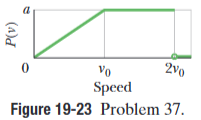
\includegraphics[width=0.25\textwidth]{picture_19-23.png} 
            % \label{fig:wrapfig}
        \end{wrapfigure}
        Figure 19-23 shows a hypothetical speed distribution for a sample of $N$ gas particles (note that $P(v) = 0$ for speed $v > 2v_0$).
        What are the values of (a) $av_0$, (b) $v_{\rm avg}/v_0$, and (c) $v_{\rm rms}/v_0$? 
        (d) What fraction of the particles has a speed between $1.5v_0$ and $2.0v_0$?

        \subsection{Solution (a)}
            We know that the total area under the curve is equal to 1.
            The area of a right triangle (like P(v) in the range of [0,$v_0$]) is $\frac{1}{2}wh$ (in this case $\frac{1}{2}av_0$), while the area of a rectangle (like P(v) in the range of [$v_0,2v_0$]) is $wh$ (in this case $av_0$).
            The total area under the curve would be the two of these added together, which we know an alternative value of.
            \begin{equation}
                \frac{3}{2}av_0 =   \int_{0}^{\infty} P(v)\,dv = 1
            \end{equation}

            Divide both sides by $av_0$ (whch we assume not to be equal to zero, which it appears not to be) and solve for $av_0$.
            \begin{gather}
                \frac{\frac{3}{2}av_0}{av_0}    =   \frac{3}{2} =   \frac{1}{av_0}\\
                \boxed{av_0    =   \frac{2}{3}}
            \end{gather}

        \subsection{Solution (b)}
            There's a formula for this.
            It can be sepaated by sections.
            \begin{align}
                v_{avg} &=  \int_{0}^{\infty} v\,P(v)\,dv
                    =   \int_{0}^{v_0} v^2 * \frac{a}{v_0}\,dv + \int_{v_0}^{2v_0} v * a \,dv + \int_{2v_0}^{\infty} v * 0\,dv\\
                    &=  \left[ \frac{v^3}{3} \cdot \frac{a}{v_0} \right]_{0}^{v_0}
                        +   \left[ \frac{v^2}{2} \cdot a \right]_{v_0}^{2v_0}
                        +   \left[ 0 \right]_{2v_0}^{\infty}\\
                    &=  \frac{av_0^2}{3} + \frac{3av_0^2}{2}
                    =   \frac{2v_0}{9} + v_0
                    =   \frac{11}{9}v_0\\
                v_{avg} / v_0   &=  \frac{11}{9}
                    =   \boxed{1.22}
            \end{align}

        \subsection{Solution (c)}
            There's a similar integral for the root-mean-square speed.
            It once again can be separated into three sections.
            \begin{align}
                v_{rms}^2   &=  \int_{0}^{\infty} v^2\,P(v)\,dv\\
                    &=  \int_{0}^{v_0} v^3 * \frac{a}{v_0}\,dv + \int_{v_0}^{2v_0} v^2 * a \,dv + \int_{2v_0}^{\infty} v^2 * 0\,dv\\
                    &=  \left[ \frac{v^4}{4} \cdot \frac{a}{v_0} \right]_{0}^{v_0}
                        +   \left[ \frac{v^3}{3} \cdot a \right]_{v_0}^{2v_0}
                        +   \left[ 0 \right]_{2v_0}^{\infty}\\
                    &=  \frac{av_0^3}{4} + \frac{7av_0^3}{3}
                    =   av_0^3 \left( \frac{1}{4} + \frac{7}{3} \right)
                    =   v_0^2 * \frac{2}{3} \left( \frac{3}{12} + \frac{28}{12} \right)\\
                    &=  v_0^2 * \left( \frac{62}{36} \right)\\
                \frac{v_{rms}}{v_0} &=  \frac{v_0}{v_0} * \frac{\sqrt{62}}{6}
                    =   \boxed{1.31}
            \end{align}

        \subsection{Solution (d)}
            Another integral is in order.
            This stuff is really just statistics at this point.
            I honestly wish that CCSF had a Probability and Statistics class that used calculus.
            Unfortunately, it doesn't.
            MATH80 doesn't require Calculus. 
            It barely even used Algebra.
            That being said, it was a great tour of what a calculator like a TI-84 Plus can do.
            \begin{align}
                \int_{1.5v_0}^{2v_0} a\,dv  &=  \left[ av \right]_{1.5v_0}^{2v_0}
                    =   a(2v_0 - 1.5v_0)
                    =   \frac{1}{2}av_0
                    =   \boxed{\frac{1}{3}}
            \end{align}

    \pagebreak
    \section{Problem 39}
        At what temperature does the rms speed of (a) $\rm H_2$ (molecular hydrogen) and (b) $\rm O_2$ (molecular oxygen) equal the escape speed from Earth (Table 13-2)? 
        At what temperature does the rms speed of (c) $\rm H_2$ and (d) $\rm O_2$ equal the escape speed from the Moon (where the gravitational acceleration at the surface has magnitude 0.16g)? 
        Considering the answers to parts (a) and (b), should there be much (e) hydrogen and (f) oxygen high in Earth's upper atmosphere, where the temperature is about 1000 K?

        \subsection{Solution (a)}
            The escape speed of earth given in table 13-2 of Halliday \& Resnick's book is 11.2 \unit{\kilo\meter/\second}.
            The molar mass of $\rm H_2$ given by table 19-1 of the same textbook is $2.02\E{-3}\,\unit{\kilo\gram/\mole}$.
            This can be used in the equation for $v_{rms}$ to find the necessary temperature for that velocity to be achieved.
            \begin{align}
                v_{rms} &=  \sqrt{\frac{3RT}{M}}\\
                T   &=  \frac{M v_{rms}^2}{3R}
                    =   \frac{2.02\E{-3}\,\unit{\kilo\gram/\mole} \cdot (11.2\E{3} \unit{\meter/\second})^2}{3 * 8.31\,\unit{\joule/\mole\cdot\kelvin}}\\
                    &=  \frac{253388.8}{24.93}\,\unit{\frac{\joule/\mole}{\joule/\mole}\cdot\kelvin}
                    =   \boxed{10164\,\unit{\kelvin}}
            \end{align}

        \subsection{Solution (b)}
            The molar mass of $\rm O_2$ given by table 19-1 of the same textbook is $32.0\E{-3}\,\unit{\kilo\gram/\mole}$.
            This can be used in the equation for $v_{rms}$ to find the necessary temperature for escape velocity to be achieved.
            \begin{align}
                v_{rms} &=  \sqrt{\frac{3RT}{M}}\\
                T   &=  \frac{M v_{rms}^2}{3R}
                    =   \frac{32.0\E{-3}\,\unit{\kilo\gram/\mole} \cdot (11.2\E{3} \unit{\meter/\second})^2}{3 * 8.31\,\unit{\joule/\mole\cdot\kelvin}}\\
                    &=  \frac{4014080}{24.93}\,\unit{\frac{\joule/\mole}{\joule/\mole}\cdot\kelvin}
                    =   \boxed{161014\,\unit{\kelvin}}
            \end{align}

        \subsection{Solution (c)}
            The escape speed of earth's moon given in table 13-2 of Halliday \& Resnick's book is 2.38 \unit{\kilo\meter/\second}.
            The molar mass of $\rm H_2$ given by table 19-1 of the same textbook is $2.02\E{-3}\,\unit{\kilo\gram/\mole}$.
            This can be used in the equation for $v_{rms}$ to find the necessary temperature for escape velocity to be achieved.
            \begin{align}
                v_{rms} &=  \sqrt{\frac{3RT}{M}}\\
                T   &=  \frac{M v_{rms}^2}{3R}
                    =   \frac{2.02\E{-3}\,\unit{\kilo\gram/\mole} \cdot (2.38\E{3} \unit{\meter/\second})^2}{3 * 8.31\,\unit{\joule/\mole\cdot\kelvin}}\\
                    &=  \frac{1142.088}{24.93}\,\unit{\frac{\joule/\mole}{\joule/\mole}\cdot\kelvin}
                    =   \boxed{458.9686\,\unit{\kelvin}}
            \end{align}

        \subsection{Solution (d)}
            The molar mass of $\rm O_2$ given by table 19-1 of the same textbook is $32.0\E{-3}\,\unit{\kilo\gram/\mole}$.
            This can be used in the equation for $v_{rms}$ to find the necessary temperature for escape velocity to be achieved.
            \begin{align}
                v_{rms} &=  \sqrt{\frac{3RT}{M}}\\
                T   &=  \frac{M v_{rms}^2}{3R}
                    =   \frac{32.0\E{-3}\,\unit{\kilo\gram/\mole} \cdot (2.38\E{3} \unit{\meter/\second})^2}{3 * 8.31\,\unit{\joule/\mole\cdot\kelvin}}\\
                    &=  \frac{181260.8}{24.93}\,\unit{\frac{\joule/\mole}{\joule/\mole}\cdot\kelvin}
                    =   \boxed{7270.79\,\unit{\kelvin}}
            \end{align}

        \subsection{Solution (e)}
            Calculate the expected rms velocity at 1000 \unit{\kelvin}.
            \begin{align}
                v_{rms} &=  \sqrt{\frac{3RT}{M}}
                    =   \sqrt{\frac{3 * 8.31 * 1000}{2.02\E{-3}}}\\
                    &=  \sqrt{\frac{24.93\E{6}}{2.02}}
                    =   \sqrt{12.34\E{6}}\\
                    &=  3.51\E{3} \unit{\meter/\second}
            \end{align}

            There should be some hydrogen up there, but a lot of it would have likely escaped since 3.51 is not excessively smaller than 11.2. 
            The answer is \boxed{no}.

        \subsection{Solution (f)}
            Calculate the expected rms velocity at 1000 \unit{\kelvin}.
            \begin{align}
                v_{rms} &=  \sqrt{\frac{3RT}{M}}
                    =   \sqrt{\frac{3 * 8.31 * 1000}{32.00\E{-3}}}\\
                    &=  \sqrt{\frac{24.93\E{6}}{32.00}}
                    =   \sqrt{0.779\E{6}}\\
                    &=  0.88\E{3} \unit{\meter/\second}
            \end{align}

            There should be a fair amount of hydrogen up there, even if a little of it would have escaped since 0.88 is much smaller than 11.2. 
            The answer is \boxed{yes}.

    \pagebreak
    \section{Problem 43}
        The temperature of 3.00 mol of an ideal diatomic gas is increased by 40.0 \unit{\celsiusdegree} without the pressure of the gas changing.
        The molecules in the gas rotate but do not oscillate. 
        (a) How much energy is transferred to the gas as heat? 
        (b) What is the change in the internal energy of the gas? 
        (c) How much work is done by the gas? 
        (d) By how much does the rotational kinetic energy of the gas increase?

        \subsection{Solution (a)}
            We have an equation for the energy transfered to the gas as heat.
            \begin{align}
                C_P &=  C_V + R
                    =   20.8\,\unit{\joule/\mole\cdot\kelvin} + 8.31\,\unit{\joule/\mole\cdot\kelvin}
                    =   29.11\,\unit{\joule/\mole\cdot\kelvin}\\
                Q   &=  nC_P \Delta T
                    =   3.00\,\unit{\mole} * 29.11\,\unit{\joule/\mole\cdot\kelvin} * 40\,\unit{\kelvin}\\
                    =   \boxed{3493.2,\unit{\joule}}
            \end{align}

        \subsection{Solution (b)}
            We have an equation for the work done on the gas.
            \begin{align}
                W   &=  -nR\Delta T
                    =   -3.00\unit{\mole} * 8.31\unit{\joule/\mole\cdot\kelvin} * 40.0\unit{\kelvin}\\
                    &=  -997.2\,\unit{\joule}
            \end{align}

            The first law of thermodynamics can guide us from here.
            \begin{align}
                \Delta E_{int}  &=  Q_{\rm in} + W_{\rm in}
                    =   3493.2\,\unit{\joule} - 997.2\,\unit{\joule}\\
                    &=  \boxed{2496\,\unit{\joule}}
            \end{align}
        
        \subsection{Solution (c)}
            The work done by the gas is the aforementioned \boxed{997.2\,\unit{\joule}}

        \subsection{Solution (d)}
            The rotational kinetic energy is the kinetic energy added that would not be translational.
            There is a formula for the translational kinetic energy, and we already know the change in the total energy.
            \begin{align}
                \Delta E_{int}  &=  \Delta K_{\rm rot} + \Delta K_{\rm tra}\\
                \Delta K_{\rm rot}  &=  \Delta E_{int} - \Delta K_{\rm tra}
                    =   2496\,\unit{\joule} - \frac{3}{2}Nk*40\,\unit{\celsiusdegree}\\
                    &=  2496\,\unit{\joule} - \frac{3}{2}(n*N_A)k*40\,\unit{\celsiusdegree}\\
                    &=  2496\,\unit{\joule} - \frac{3}{2} * 1.38\E{-23} * 3.0 * 6.022\E{23} * 40\,\unit{\kelvin}\\
                    &=  2496\,\unit{\joule} - 1496\,\unit{\joule}
                    =   \boxed{1000\,\unit{\joule}}
            \end{align}
            

    \pagebreak
    \section{Problem 45}
        The mass of a gas molecule can be computed from its specific heat at constant volume $c_V$ (note that this is not $C_V$). 
        Take $c_V = 0.075 \unit{\calorie/\gram\cdot\celsiusdegree}$ for argon and calculate (a) the mass of an argon atom and (b) the molar mass of argon.

        \subsection{Solution}

    \pagebreak
    \section{Problem 47}
        The temperature of $2.00 \unit{\mole}$ of an ideal monatomic gas is raised 15.0 K at constant volume. 
        What are (a) the work W done by the gas, (b) the energy transferred as heat Q, (c) the change $\Delta E_{\rm int}$ in the internal energy of the gas, and (d) the change $\Delta K$ in the average kinetic energy per atom?

        \subsection{Solution}

    \pagebreak
    \section{Problem 51}
        When 1.0 mol of oxygen ($O_2$) gas is heated at constant pressure starting at 0°C, how much energy must be added to the gas as heat to double its volume? 
        The molecules rotate but do not oscillate.

        \subsection{Solution}

    \pagebreak
    \section{Problem 55}

        \subsection{Solution}

    \pagebreak
    \section{Problem 57}

        \subsection{Solution}

    \pagebreak
    \section{Problem 59}

        \subsection{Solution}

    \pagebreak
    \section{Problem 63}

        \subsection{Solution}

    \pagebreak
    \section{Problem 69}

        \subsection{Solution}

    \pagebreak
    \section{Problem 75}

        \subsection{Solution}

    \pagebreak
    \section{Problem 77}

        \subsection{Solution}

    \pagebreak
    
    \tableofcontents
\end{document}